% !TeX root = ../main.tex

\chapter{Recommendation Generation}\label{chapter:recommendation-generation}

This chapter introduces the recommendation generation component of the prototype through an incremental perspective. Instead of presenting the full recommendation workflow at once, the chapter is structured around the main building blocks that progressively establish a grounded and inspectable recommendation process. It first introduces the data foundation on which recommendation output is based. It then outlines the framework used to evaluate how the system reasons during recommendation generation.

\section{Data Grounding for Recommendation Generation}\label{section:recommendation-generation:data-grounding}

The recommendation component is grounded in a destination catalogue that is based on the dataset used in Sarica's DestiRec thesis~\parencite{saricaDestirec}. In the current prototype, this catalogue acts as the primary structured source from which destinations can be filtered, compared, and ranked. This grounding constraint is important for the overall system design. The prototype can only recommend destinations that are explicitly represented in this catalogue, and it can only reason over preference dimensions that are encoded in the available attributes.

For the recommendation generation approach considered in this thesis, the dataset provides 163 usable destination regions that form the grounding basis of the system.

\subsection{Schema and Value Encoding}\label{subsection:recommendation-generation:data-grounding:schema}

The dataset combines identification fields, cost information, temporal suitability fields, and thematic descriptors. \autoref{table:recommendation-generation:schema-overview} summarizes the schema used for recommendation generation.

\begin{table}[htbp]
\centering
\begin{tabular}{p{0.24\linewidth}p{0.23\linewidth}p{0.43\linewidth}}
\hline
Field & Value type & Description \\
\hline
\texttt{parent\_region} & text & Broad geographic grouping of a destination region \\
\texttt{region} & text & Name of the destination region \\
\texttt{u\_name} & text code & Unique identifier of the destination region \\
\texttt{cost\_per\_week} & numeric value & Estimated weekly travel cost \\
\texttt{popularity} & ordinal scale & General popularity indicator of the destination region \\
\texttt{jan} to \texttt{dec} & ordinal scale & Month-specific suitability values from January to December \\
\texttt{safety} & ordinal scale & Safety-related characterization of the destination region \\
\texttt{nature} & ordinal scale & Strength of nature-oriented travel characteristics \\
\texttt{hiking} & ordinal scale & Strength of hiking-related travel characteristics \\
\texttt{beach} & ordinal scale & Strength of beach-related travel characteristics \\
\texttt{watersports} & ordinal scale & Strength of water-sport-related travel characteristics \\
\texttt{entertainment} & ordinal scale & Strength of entertainment-oriented travel characteristics \\
\texttt{wintersports} & ordinal scale & Strength of winter-sport-related travel characteristics \\
\texttt{culture} & ordinal scale & Strength of cultural travel characteristics \\
\texttt{culinary} & ordinal scale & Strength of food-related travel characteristics \\
\texttt{architecture} & ordinal scale & Strength of architecture-related travel characteristics \\
\texttt{shopping} & ordinal scale & Strength of shopping-related travel characteristics \\
\hline
\end{tabular}
\caption{Schema overview of the recommendation dataset}
\label{table:recommendation-generation:schema-overview}
\end{table}

The table shows that the schema combines four different layers of information. The first layer identifies and localizes the destination region. The second layer captures a direct budget signal through \texttt{cost\_per\_week}. The third layer describes when a destination is suitable through the month-specific fields. The fourth layer characterizes what kind of travel experience a region is associated with through thematic descriptors such as nature, culture, or watersports. Together, these layers provide the basic structure on which later filtering and preference interpretation operate.

Most temporal and thematic fields are not stored as raw continuous numbers. Instead, they use an \emph{ordinal scale} with the symbols \texttt{--}, \texttt{-}, \texttt{o}, \texttt{+}, and \texttt{++}. In this context, an \emph{ordinal scale} means that the values express an ordered progression from lower to higher suitability or strength, without claiming that the distance between neighboring levels is measured exactly. These symbols are mapped to the numeric values 0.0, 0.25, 0.5, 0.75, and 1.0. The same mapping is also applied to the \texttt{popularity} field. This allows the dataset to express relative strength and suitability in a comparable way across many different attributes, while still remaining coarse-grained rather than highly fine-grained.

\subsection{Hard and Soft Data Categories}\label{subsection:recommendation-generation:data-grounding:hard-soft-preferences}

For recommendation generation, it is useful to distinguish between hard and soft data categories. This distinction reflects how different parts of the dataset should influence the recommendation process when they are matched against user input. In the following work, hard preferences will be referred to as \emph{filters}, whereas soft preferences will be referred to as \emph{preferences} or \emph{user interests}.

Hard data categories are those that define the feasible search space more directly. In the present dataset, these include geographic scope through \texttt{parent\_region}, budget through \texttt{cost\_per\_week}, and seasonality through the monthly suitability fields from \texttt{jan} to \texttt{dec}. These categories are treated as hard because users often formulate them as actual constraints. If a user asks for destinations in Europe, for a limited budget, or suitable for a specific month or season, violating such conditions usually makes a recommendation substantially less useful. These attributes therefore function naturally as filters that narrow the candidate set before finer trade-offs are considered.

Soft data categories are those that describe thematic interests rather than strict feasibility constraints. In the present dataset, these include \texttt{nature}, \texttt{hiking}, \texttt{beach}, \texttt{watersports}, \texttt{entertainment}, \texttt{wintersports}, \texttt{culture}, \texttt{culinary}, \texttt{architecture}, and \texttt{shopping}. These attributes are better interpreted as signals of what kind of travel experience the user is looking for. In many realistic travel queries, such interests are not absolute requirements. A destination can still be useful even if it only partially matches them. For that reason, these categories are more suitable for ranking, weighting, and preference balancing than for strict exclusion.

This division is important for both recommendation quality and interpretability. If all attributes were treated as equally strict, the system would risk eliminating plausible destinations too early. If all attributes were treated as equally soft, the system could return destinations that violate explicit user constraints on geography, budget, or time of travel. Separating hard and soft categories therefore supports a more faithful mapping from natural language requests to recommendation logic. Filters delimit what is acceptable at all, whereas preferences or user interests determine which of the acceptable candidates is most aligned with the user's interests.

\subsection{Geographic Coverage and Granularity}\label{subsection:recommendation-generation:data-grounding:coverage}

The dataset is distributed across Europe, North America, South America, Africa, Asia, Australia, and Antarctica. More importantly, its internal structure follows travel characteristics rather than political borders alone. The regional division is designed to represent coherent travel spaces: areas with similar climate, landscape, activities, seasonality, or cultural profile can be grouped into one recommendation unit, whereas large countries can be divided into several units when different parts of the same country differ substantially along these dimensions.

\begin{table}[htbp]
\centering
\begin{tabular}{lr}
\hline
World region & Records \\
\hline
Europe & 32 \\
North America & 34 \\
South America & 17 \\
Africa & 21 \\
Asia & 50 \\
Australia & 8 \\
Antarctica & 1 \\
\hline
Total & 163 \\
\hline
\end{tabular}
\caption{Operational destination records by world region}
\label{table:recommendation-generation:destination-distribution}
\end{table}

This means that the recommendation units are intentionally not uniform at the country level. Some correspond roughly to one country, some combine several neighboring areas, and some subdivide large countries into multiple regions. They should therefore be interpreted primarily as travel regions rather than as political entities. This structure is important for recommendation generation because users usually search for a particular kind of travel experience, and the dataset is organized to express these experiential differences more clearly than a strictly country-based representation would.

\subsection{Distribution of Costs and Seasonal Signals}\label{subsection:recommendation-generation:data-grounding:distributions}

The cost field provides one of the clearest structured anchors for recommendation generation. \autoref{table:recommendation-generation:cost-groups} summarizes the main distribution statistics for the weekly cost values, both for the full dataset and across the major continental groups. Overall, the cost structure is centered in the middle range, with a mean of 485.25~EUR, a 50th percentile of 400~EUR, and a 75th percentile of 560~EUR. The gap between the mean and the median indicates that the distribution is pulled upward by a smaller number of more expensive regions.

\begin{table}[htbp]
\centering
\begin{tabular}{lrrrrr}
\hline
Region group & Min & Max & Mean & P50 & P75 \\
\hline
Overall & 250 & 4500 & 485.25 & 400 & 560 \\
Europe & 350 & 750 & 402.50 & 350 & 420 \\
North America & 250 & 975 & 564.41 & 600 & 693.75 \\
South America & 310 & 625 & 472.06 & 400 & 625 \\
Africa & 350 & 560 & 415.00 & 390 & 450 \\
Asia & 250 & 560 & 411.30 & 400 & 450 \\
Australia & 490 & 800 & 652.50 & 655 & 750 \\
Antarctica & 4500 & 4500 & 4500.00 & 4500 & 4500 \\
\hline
\end{tabular}
\caption{Weekly cost statistics overall and across region groups}
\label{table:recommendation-generation:cost-groups}
\end{table}

Across continents, the distribution is not uniform. Europe, Africa, and Asia are comparatively concentrated in the lower to middle cost range, with means close to 400~EUR and 50th percentiles between 350~EUR and 400~EUR. North America and Australia are clearly more expensive on average, with North America centered around 600~EUR and Australia even higher. Antarctica is an extreme outlier with a single very high-cost region, so it should be interpreted separately from the rest of the dataset rather than as part of the ordinary travel budget distribution.

The seasonal profile is also informative. When the monthly suitability values are mapped to their numeric equivalents and averaged across all records, the strongest months are October and September, followed closely by May and June. The weakest months are January, December, and February. This suggests that the dataset is structurally strongest for spring, summer, and early autumn travel. 

\subsection{Thematic Profile}\label{subsection:recommendation-generation:data-grounding:limitations}

The thematic profile of the dataset is defined through the soft categories \texttt{nature}, \texttt{hiking}, \texttt{beach}, \texttt{watersports}, \texttt{entertainment}, \texttt{wintersports}, \texttt{culture}, \texttt{culinary}, \texttt{architecture}, and \texttt{shopping}. These categories describe different thematic aspects of a destination region and characterize the kinds of experiences associated with it.

Taken together, these categories cover several complementary dimensions of travel. Some fields focus on outdoor and landscape-oriented experiences, especially \texttt{nature}, \texttt{hiking}, and \texttt{wintersports}. Others capture coastal and water-oriented travel through \texttt{beach} and \texttt{watersports}. A third group reflects urban and cultural experiences through \texttt{culture}, \texttt{architecture}, and \texttt{entertainment}. Finally, \texttt{culinary} and \texttt{shopping} represent forms of destination appeal that are tied less to geography alone and more to local atmosphere, consumption, and city or regional lifestyle.

The categories therefore span a broad range of travel themes, from nature-oriented and activity-oriented travel to urban, cultural, and lifestyle-oriented travel. They describe destination regions not through one single theme, but through a combination of thematic dimensions that can coexist within the same region.

At the same time, the categories are intentionally broad. They do not attempt to represent every niche activity or every subtle distinction between destinations. Instead, they provide a compact thematic characterization of regions at a level that remains general enough to be applied consistently across the full dataset.

\section{Technology Used for Recommendation Generation}\label{section:recommendation-generation:technology}

\subsection{Framework Basis}

The recommendation workflow in the developed system is implemented in Python through a combination of the LangChain and LangGraph frameworks. LangChain provides the higher-level components for building language-model-based application logic, especially the integration of models, prompts, and tool-oriented agent behavior~\parencite{langchainOverview}. LangGraph provides the lower-level orchestration layer for building stateful agent workflows as explicit graphs with controlled transitions between processing steps~\parencite{langgraphOverview}. In the present system, LangChain is therefore used mainly for agent construction, while LangGraph is used mainly for execution structure and control flow.

\subsection{Graph-Based Workflow Concepts}

In the context of this system, a \emph{graph} is the overall recommendation workflow represented as a directed processing structure. It defines which steps exist, how state moves between them, and under which conditions the workflow branches, continues, or terminates. A \emph{node} is one executable step inside this graph. Nodes perform concrete tasks such as loading conversation state, routing the request, synthesizing the user request, extracting filters, generating recommendations, or producing the final response. An \emph{agent} is the language-model-based decision component used within some of these nodes. In this system, agents are responsible for tasks that require interpretation or generation, such as request routing, filter extraction, synthesized-query construction, and response generation. In this sense, the agent does not represent the whole application. Rather, it is one reasoning component embedded within a broader graph-based workflow.

\subsection{Storage and Data Access}

The destination data used during recommendation generation is stored in a SQL database. This is used as a functional storage engine that keeps the travel destination data in one location and allows access through standard SQL queries over the destination table and its structured attributes.

\section{System Reasoning Evaluation Framework}\label{section:recommendation-generation:reasoning-evaluation-framework}

The system reasoning evaluation framework considered here focuses on the single-turn setting. Its purpose is to understand how a given recommendation architecture handles extraction and reasoning for single-shot travel queries. In this context, the term \emph{filter} refers to the hard categories defined in \autoref{subsection:recommendation-generation:data-grounding:hard-soft-preferences}, namely geographic scope, budget, and seasonality. The term \emph{preference} or \emph{user interest} refers to the soft thematic categories introduced in the same subsection.

Methodologically, the framework varies these two dimensions independently. One axis controls how clearly filters are expressed in a query. The other axis controls how specifically preferences are formulated. This makes it possible to observe whether a system architecture can identify filters and preferences under increasingly explicit or increasingly narrow query formulations, while the overall task remains the same.

The field symbols used in the framework are summarized in \autoref{table:recommendation-generation:reasoning-matrix-legend}. The three filter levels range from no explicit filter signal to explicit machine-checkable constraints. The three preference levels range from broad thematic interests to highly specialized travel intents. In addition, the evaluation contains a separate unrelated-query category for inputs that do not belong to the travel recommendation task at all.

\begin{table}[htbp]
\centering
\begin{tabular}{p{0.1\linewidth}p{0.18\linewidth}p{0.32\linewidth}p{0.26\linewidth}}
\hline
Symbol & Name & Description & Example \\
\hline
F0 & No Filter & No explicit continent, budget, or season is stated. & ``I want to travel somewhere nice.'' \\
F1 & Vague Filter & A filter signal is present, but only indirectly or weakly expressed. & ``without spending a fortune'' \\
F2 & Explicit Filter & Continent, budget, season, or several of them are stated in a machine-checkable form. & ``Europe this summer for under \$1500'' \\
P0 & Very Vague Preference & Only a broad interest is stated, such as beach, food, mountains, or city travel. & ``Looking for a big city where I can walk around all day.'' \\
P1 & Experience-Focused Preference & The query points to a recognizable travel experience without becoming highly narrow. & ``Point me to a place where I can just drink amazing wine by a vineyard all day.'' \\
P2 & Highly Specialized Preference & The intended experience is narrow and tied to a specific activity, landmark, place, food, or object. & ``Where is the best spot to go scuba diving with manta rays?'' \\
U & Unrelated Query & The input is outside the system's intended travel recommendation scope and should not be interpreted as a normal recommendation request. & ``How do I reset my laptop password?'' \\
\hline
\end{tabular}
\caption{Interpretation of the single-turn matrix symbols}
\label{table:recommendation-generation:reasoning-matrix-legend}
\end{table}

The full evaluation matrix is obtained by combining one filter level with one preference level. This results in nine travel-related cells, shown in \autoref{table:recommendation-generation:reasoning-matrix}. A query in \texttt{F0\_P0} is open and weakly structured because it contains neither explicit filters nor a narrowly defined interest. A query in \texttt{F1\_P1} combines weak filter hints with a more recognizable experience. A query in \texttt{F2\_P2} combines explicit filters with a highly specialized travel intent. The matrix therefore creates controlled variation in single-turn reasoning difficulty while keeping the task domain constant.

\begin{table}[htbp]
\centering
\small
\setlength{\tabcolsep}{4pt}
\begin{tabular}{p{0.17\linewidth}p{0.25\linewidth}p{0.25\linewidth}p{0.25\linewidth}}
\hline
 & P0 Very Vague Preference & P1 Experience-Focused Preference & P2 Highly Specialized Preference \\
\hline
F0 No Filter & broad interest without explicit filters & concrete experience without explicit filters & narrow interest without explicit filters \\
F1 Vague Filter & vague filter with broad interest & vague filter with concrete experience & vague filter with highly specialized interest \\
F2 Explicit Filter & explicit filter with broad interest & explicit filter with concrete experience & explicit filter with highly specialized interest \\
\hline
\end{tabular}
\caption{Single-turn reasoning evaluation matrix}
\label{table:recommendation-generation:reasoning-matrix}
\end{table}

To instantiate this matrix, a synthetic single-turn evaluation set was generated with GPT-5.4. The generation process followed a dedicated prompt specification documented in \texttt{backend/src/evaluation/test\_data\_generation\_plan.md}. The same matrix is used across the compared system versions, each matrix cell contains 100 entries, and a separate set of 100 unrelated queries is kept outside the main matrix. These unrelated queries are included to assess how the system handles inputs that are outside its intended scope of purpose, namely cases that should not be processed as travel recommendation requests at all. As a result, the single-turn set contains 900 travel-related evaluation queries and an additional 100 unrelated queries. The queries were intentionally written in varied and non-templated language so that the evaluation captures reasoning over diverse formulations rather than recognition of repeated phrasing.
% TODO: Add the full GPT-5.4 generation prompt in the appendix.

This evaluation data is intended to provide a better understanding of how a given system architecture reasons about a single user request. It does not aim to validate the final recommendation list as such, nor to judge the overall quality of the returned recommendations. Instead, the focus is on whether the system can identify and extract active filters and active user interests from one query, and on how clearly this reasoning becomes observable in different architectural setups. In this sense, the framework is aimed at reasoning analysis for single-shot queries rather than at end-to-end recommendation validation.

The same evaluation data is run across different recommendation architectures with different capabilities so that reasoning behavior can be compared under identical input conditions. This includes architectures that expose little internal structure as well as architectures that produce more explicit intermediate reasoning and extraction steps. In addition, the evaluation is executed with both a locally runnable open-source model via Ollama, namely Llama~3.1 with 8B parameters, and the commercial model GPT-4o. These two models were chosen in order to compare a smaller local open-source model with a commercial model, to make the evaluation results more objective, and to avoid limiting the analysis to a single underlying model.

\section{Recommender V1.0}\label{section:recommendation-generation:architecture-v1-0}

Recommender V1.0 is the earliest graph-based recommendation workflow used in the system. It is intentionally simple and consists of one agent and one database-query tool embedded in a small iterative LangGraph workflow. The purpose of this version is to let the agent interpret the user request, turn this interpretation into a structured query over the destination data, inspect the returned candidate regions, and then either continue the search by refining the query or finish with a response.

\begin{figure}[htbp]
\centering
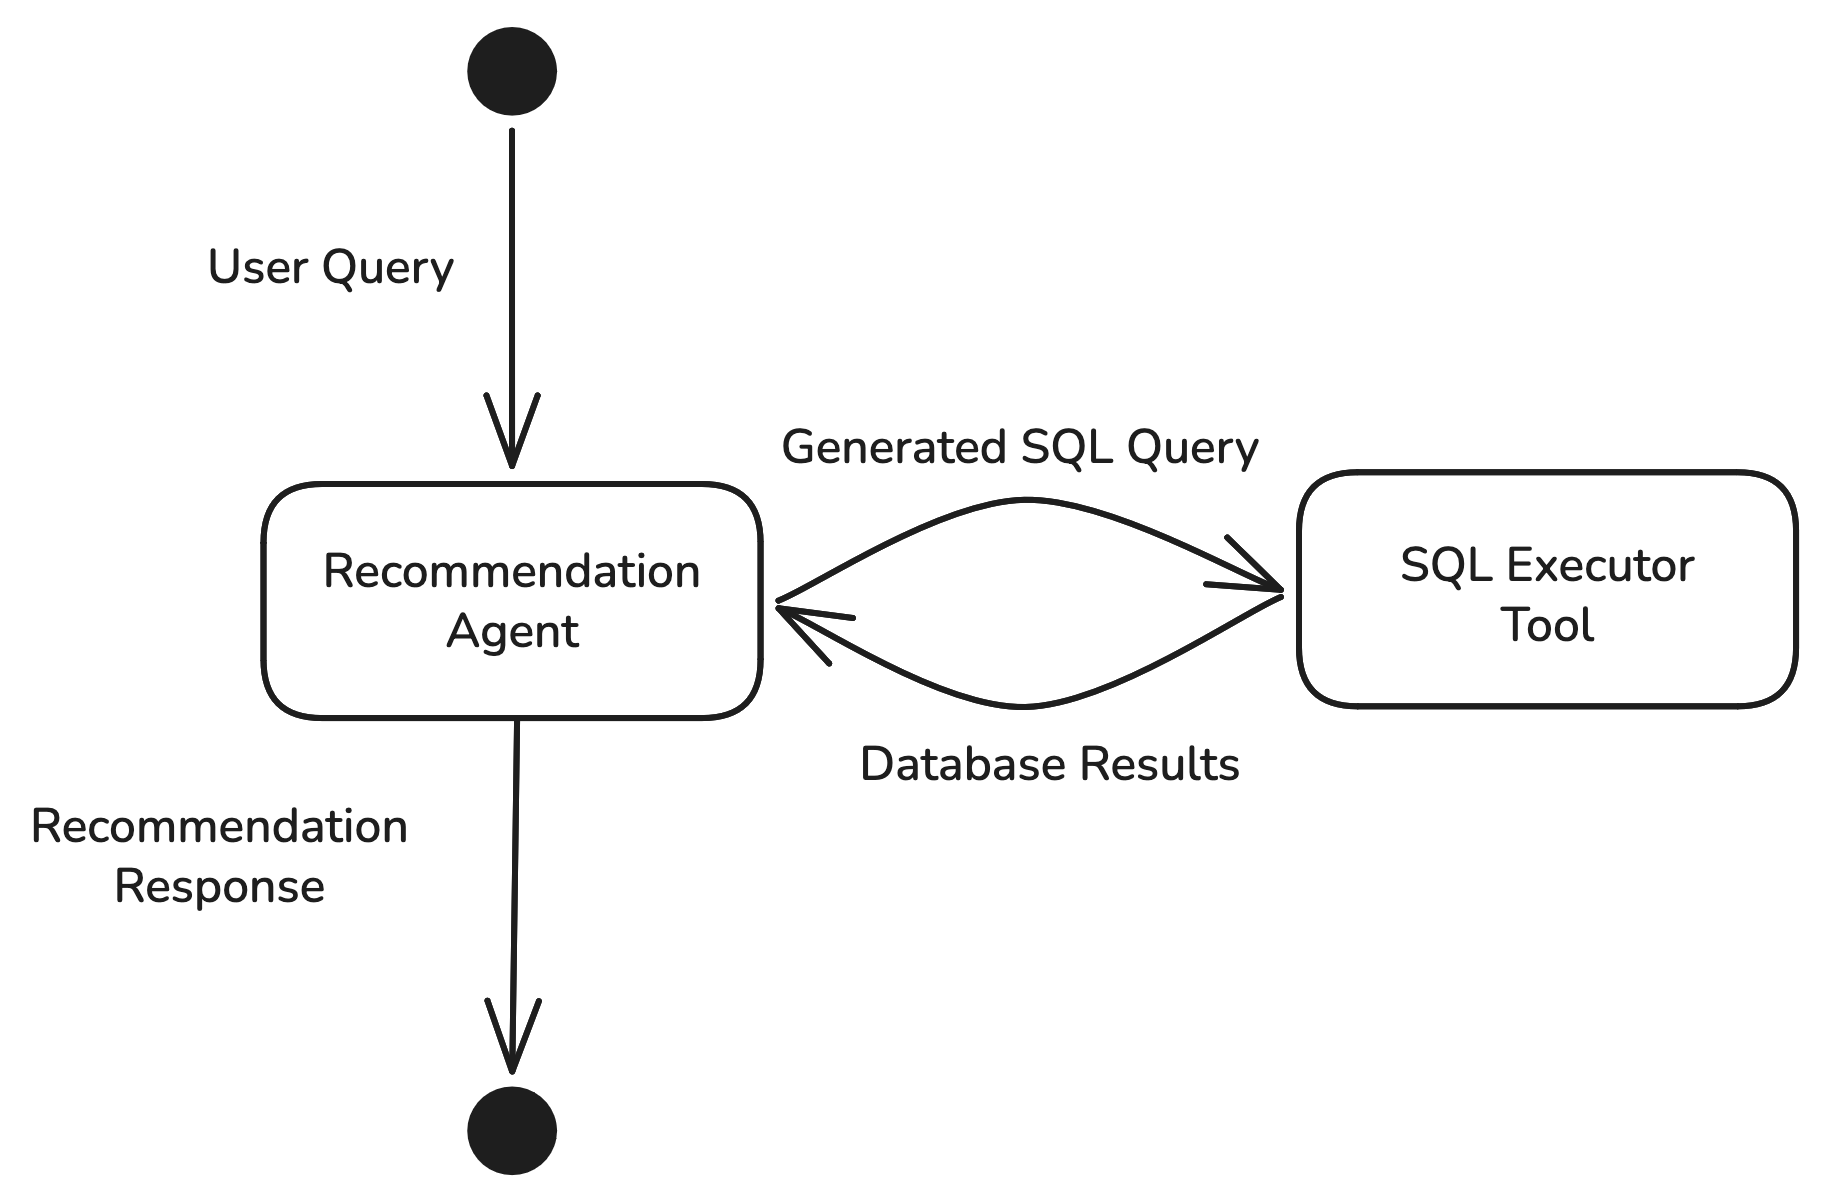
\includegraphics[width=0.9\linewidth]{figures/recommendation_v10_graph.png}
\caption{System diagram of Recommender V1.0}
\label{figure:recommendation-generation:v1-0-graph}
\end{figure}

At the graph level, the workflow is centered on an agent-tool loop. The recommendation agent node receives the current user request and decides whether to request one tool execution or to finish the run with a final response and a list of recommendations. If a tool request is produced, execution is routed to the SQL tool node. The tool result is then passed back to the recommendation-agent node, so that the agent can either issue another query or finish the run.

The remainder of the architecture is deliberately minimal. The agent has access to one read-only retrieval tool, \texttt{query\_travel\_destinations\_sql}, which operates over the \texttt{travel\_destinations} table. Recommendation generation is therefore centered on one core operation: translating the interpreted user request into explicit SQL-based retrieval over structured destination attributes.

The prompting strategy in V1.0 follows a ReAct-like pattern. The prompt frames the model as a general-purpose agent that must alternate between two actions: request one tool step or finish with a final recommendation response. It explicitly describes the available destination-table fields, states that tool results are the only admissible evidence for final recommendations, and instructs the agent to use the latest user request as the main trigger. It also encourages an iterative search strategy: first formulate the travel intent, then retrieve supporting evidence, and finally respond only when the available candidates are sufficient, as formalized in the V1.0 prompt implementation~\parencite{v10RecommenderPrompt}.

In practice, this means that V1.0 handles both filters and preferences through query construction rather than through separate extraction stages. The architecture exposes its reasoning mainly through the SQL query requested by the agent and through the sequence of tool decisions that follow from it. For that reason, V1.0 serves as a compact baseline for examining how far a single agent with one structured retrieval tool can carry the recommendation process.

\subsection{Results on the Synthetic Single-Turn Queries}\label{subsection:recommendation-generation:recommender-v1-0-results}

The synthetic single-turn evaluation set~\parencite{syntheticSingleTurnEval} was run for Recommender V1.0 with two underlying models: Llama~3.1 8B and GPT-4o. For this recommender, the most immediate comparison criterion is the rate of technically successful runs, because the architecture depends on explicit tool requests and explicit query construction. A run is therefore counted as successful when the workflow finishes without execution error, regardless of whether it returns recommendations or ends with an empty result. The overall comparison is summarized in \autoref{table:recommendation-generation:v1-0-overall-success}.

\begin{table}[htbp]
\centering
\begin{tabular}{lrrrr}
\hline
Model & Queries & Successful runs & Error runs & Success rate \\
\hline
Llama~3.1 8B & 1000 & 703 & 297 & 70.3\% \\
GPT-4o & 1000 & 998 & 2 & 99.8\% \\
\hline
\end{tabular}
\caption{Overall execution success of Recommender V1.0 on the synthetic single-turn queries}
\label{table:recommendation-generation:v1-0-overall-success}
\end{table}

The contrast is substantial. GPT-4o remains almost fully stable across the synthetic evaluation, whereas the Llama-based variant fails in nearly one third of all runs. This difference indicates that the main weakness of V1.0 is not only the retrieval design itself, but also the stability of the model when it must repeatedly formulate valid tool requests and valid structured queries.

The error traces show that these failures are closely tied to SQL-query assembly and tool-use control. In the Llama-based runs, the dominant failure modes are missing SQL queries in tool requests and attempts to request another tool step in a final round where no further tool action is allowed. In addition, there are repeated SQL errors caused by invalid field references, malformed SQL syntax, and invalid value typing inside SQL conditions. The GPT-4o runs show only two recorded failures, one SQL syntax failure and one SQL error caused by an invalid column reference.

\begin{table}[htbp]
\centering
\begin{tabular}{lrr}
\hline
Error category & Llama~3.1 8B & GPT-4o \\
\hline
Missing \texttt{sql\_query} in tool request & 121 & 0 \\
Tool request issued in final round & 121 & 0 \\
Invalid SQL column reference & 39 & 1 \\
SQL syntax error & 11 & 1 \\
Invalid SQL value or type usage & 3 & 0 \\
Invalid SQL operator or function usage & 1 & 0 \\
Missing final response after finish & 1 & 0 \\
\hline
Total & 297 & 2 \\
\hline
\end{tabular}
\caption{Observed V1.0 execution errors by category}
\label{table:recommendation-generation:v1-0-error-categories}
\end{table}

These results suggest that the V1.0 architecture is highly sensitive to the model's ability to follow the prompt protocol and to formulate structurally valid SQL-oriented actions. For this reason, the execution-success comparison is already informative in itself. Before interpreting how well filters or preferences are captured, it is necessary to establish whether the architecture can reliably sustain the agent-tool loop without breaking its own query-construction logic. In the case of V1.0, this requirement is satisfied much more consistently by GPT-4o than by the smaller Llama model.

For the travel-related matrix queries, the result traces can be examined more directly through the SQL behavior that the architecture exposes. In this case, the analysis is necessarily approximate, because V1.0 does not externalize separate filter-extraction or preference-extraction structures. Instead, both become visible only through the SQL query requested by the agent. The counts below are therefore derived from successful runs only and were assigned manually by expert inspection of the result traces. A run is counted as having produced recommendations when it finishes with a non-empty recommendation list. A filter is counted as correctly identified when the SQL query preserves the expected hard constraints of the request. A preference is counted as mapped when the SQL query contains a visible proxy for the intended travel interest, for example through thematic fields such as \texttt{beach}, \texttt{nature}, \texttt{culinary}, or \texttt{culture}, or through a direct region-oriented substitute. This should be understood as an operational approximation of the architecture's observable reasoning rather than as a semantic judgment of recommendation quality.

\begin{table}[htbp]
\centering
\begin{tabular}{lrrrr}
\hline
Cell & Success & Recs. returned & Filters correct & Preference mapped \\
\hline
\texttt{F0\_P0} & 90 & 59 & 73 & 88 \\
\texttt{F0\_P1} & 78 & 46 & 62 & 78 \\
\texttt{F0\_P2} & 76 & 21 & 31 & 76 \\
\texttt{F1\_P0} & 100 & 98 & 44 & 91 \\
\texttt{F1\_P1} & 76 & 58 & 52 & 74 \\
\texttt{F1\_P2} & 68 & 27 & 20 & 63 \\
\texttt{F2\_P0} & 72 & 54 & 70 & 72 \\
\texttt{F2\_P1} & 44 & 24 & 30 & 44 \\
\texttt{F2\_P2} & 60 & 40 & 46 & 60 \\
\hline
\end{tabular}
\caption{Approximate matrix-level behavior of Recommender V1.0 with Llama~3.1 8B}
\label{table:recommendation-generation:v1-0-llama-matrix-analysis}
\end{table}

\begin{table}[htbp]
\centering
\begin{tabular}{lrrrr}
\hline
Cell & Success & Recs. returned & Filters correct & Preference mapped \\
\hline
\texttt{F0\_P0} & 100 & 96 & 87 & 92 \\
\texttt{F0\_P1} & 100 & 87 & 80 & 93 \\
\texttt{F0\_P2} & 99 & 19 & 66 & 58 \\
\texttt{F1\_P0} & 100 & 95 & 52 & 91 \\
\texttt{F1\_P1} & 100 & 96 & 69 & 98 \\
\texttt{F1\_P2} & 100 & 30 & 20 & 68 \\
\texttt{F2\_P0} & 100 & 95 & 99 & 99 \\
\texttt{F2\_P1} & 99 & 89 & 95 & 95 \\
\texttt{F2\_P2} & 100 & 64 & 94 & 98 \\
\hline
\end{tabular}
\caption{Approximate matrix-level behavior of Recommender V1.0 with GPT-4o}
\label{table:recommendation-generation:v1-0-gpt-matrix-analysis}
\end{table}

These tables show a clear structural difference between the two model variants. GPT-4o is not only more stable overall, but also more consistent in translating the hard constraints of the query into SQL clauses. This becomes especially visible in the explicit-filter cases \texttt{F2\_P0}, \texttt{F2\_P1}, and \texttt{F2\_P2}, where correct filter handling is high and incorrect filter insertion is rare. The Llama-based variant, by contrast, shows a much weaker pattern in the same cells, even when the run itself completes successfully. This suggests that successful execution alone is not enough to guarantee coherent filter translation.

\begin{table}[htbp]
\centering
\begin{tabular}{lrr}
\hline
Measure & Llama~3.1 8B & GPT-4o \\
\hline
Recommendation rate & 64.3\% & 74.7\% \\
Filter-correct rate & 64.5\% & 73.7\% \\
Preference-mapped rate & 83.6\% & 88.2\% \\
\hline
\end{tabular}
\caption{Aggregate matrix-level rates of Recommender V1.0 across successful runs}
\label{table:recommendation-generation:v1-0-aggregate-matrix-rates}
\end{table}

At the aggregate level, GPT-4o produces recommendations more often and preserves the expected hard constraints more often. The difference in preference mapping is smaller. This suggests that even the smaller model often finds some structured proxy for the user interest, but is less reliable in translating the full set of hard constraints into coherent SQL.

The preference column should be interpreted more cautiously. Because V1.0 represents preferences only through SQL query construction, the presence of a thematic mapping mainly shows that the architecture found a structured proxy for the user interest. In broad cases such as \texttt{P0}, this often works well because the request can be mapped to fields such as \texttt{beach}, \texttt{nature}, \texttt{hiking}, or \texttt{culinary}. In more specific cases, especially \texttt{P2}, the preference is often reduced to a broader proxy or to a literal region match. The tables therefore do not show whether the full nuance of the preference was preserved, but they do show whether the architecture was able to turn the request into some structured representation at all.

\begin{table}[htbp]
\centering
\begin{tabular}{lrrr}
\hline
Model & Queries & Successful runs & Valid scope responses \\
\hline
Llama~3.1 8B & 100 & 39 & 24 \\
GPT-4o & 100 & 100 & 100 \\
\hline
\end{tabular}
\caption{Successful-run rates of Recommender V1.0 on unrelated queries}
\label{table:recommendation-generation:v1-0-unrelated-success}
\end{table}

The unrelated-query set should be interpreted separately because it does not test destination reasoning, but scope handling. In this context, a valid scope response means that the system finishes successfully and returns no recommendations for an out-of-scope input. Here the contrast is even sharper. GPT-4o completes all 100 unrelated-query runs without execution error and produces a valid scope response in all cases. The Llama-based variant completes only 39 of 100 successfully, and only 24 of these runs end with a valid scope response without recommendations. This means that the weaker model is not only less stable on travel-related reasoning, but also less reliable when the architecture is forced to reject or deflect requests that are outside the intended recommendation scope.

Beyond execution success, the result traces also show how V1.0 captures filters. In this architecture, filters are not extracted into dedicated intermediate structures. Instead, they become visible through the SQL clauses requested by the agent. When the user provides no explicit filters, as in \texttt{F0}, GPT-4o usually avoids hard geographic or budget constraints and formulates mainly thematic SQL conditions such as \texttt{beach > 0.8} or \texttt{nature > 0.7 AND hiking > 0.7}. This suggests that the architecture can keep broad preferences in view without unnecessarily inventing explicit filters. In \texttt{F1}, vague filters are often normalized into approximate SQL constraints, for example by mapping ``without spending a fortune'' to a low cost threshold or by turning ``warmer months'' into summer-month conditions. In \texttt{F2}, the GPT-based variant usually translates explicit region, budget, and season constraints directly into SQL, for example through \texttt{parent\_region = 'Europe'}, \texttt{cost\_per\_week <= ...}, and month-based season clauses.

The Llama-based variant follows the same general strategy, but with noticeably lower reliability. For broad queries it often produces the expected thematic SQL restriction. However, for more explicit or more complex requests it more frequently introduces wrong month logic, incomplete query clauses, or syntactically invalid SQL. The high number of missing-\texttt{sql\_query} and final-round tool-request errors shows that filter handling in this variant breaks down not only at the level of semantic interpretation, but already at the level of tool-control discipline.

Preference capture in V1.0 follows the same SQL-centered logic. Broad preferences from \texttt{P0} are usually mapped to one or two thematic fields, for example \texttt{beach}, \texttt{nature}, \texttt{hiking}, or \texttt{culinary}. This works relatively naturally because the dataset already offers direct schema fields for such themes. In \texttt{P1}, the architecture still captures the request, but often only through proxies. Ancient ruins may be translated into \texttt{culture} or \texttt{architecture}, a wine-region request into \texttt{culinary}, and an indie music scene into \texttt{entertainment}. This means that the broader experience is often retained, but only after being compressed into the limited field vocabulary of the destination table.

The strongest limitation appears in \texttt{P2}. Highly specialized requests are often flattened into either broad thematic proxies or literal region-matching attempts. In the GPT-based runs this can still produce coherent SQL, but the resulting query may already lose the original anchor by reducing it to culture, watersports, or one exact region name. In the Llama-based runs, the same type of specialization is more likely to produce malformed SQL or unstable query refinement. As a result, V1.0 can capture broad and moderately specific preferences to a limited degree, but its handling of narrow, anchor-specific user intents remains structurally weak because the architecture forces these intents into direct SQL retrieval over a relatively small set of structured fields.

\subsection{Limitations of Recommender V1.0}\label{subsection:recommendation-generation:recommender-v1-0-limitations}

The analysis of Recommender V1.0 shows several structural limitations. The first limitation is architectural fragility. Because the recommender depends on explicit tool requests and explicit SQL construction, its behavior is highly sensitive to whether the underlying model can follow the tool protocol and produce valid structured queries. The observed runtime failures, missing SQL requests, and malformed SQL statements show that this dependency is substantial, especially for the smaller model.

The second limitation concerns how filters and preferences are represented internally. In V1.0, there is no dedicated intermediate layer for extracting or storing filters and no separate representation for user preferences. Instead, both are compressed directly into SQL constraints. This makes the architecture compact, but it also means that interpretation and retrieval are tightly coupled. As soon as the interpretation is imperfect, the retrieval logic is affected immediately, with little opportunity for later correction.

The third and more fundamental limitation concerns the treatment of user preferences expressed in natural language. In practice, V1.0 often flattens a user request into one or a few broad schema fields such as \texttt{culture}, \texttt{culinary}, \texttt{nature}, or \texttt{watersports}. This defeats an important part of the purpose of natural, unrestricted language input. Although the user can formulate a request in a nuanced and open-ended way, the architecture ultimately reduces this request to a limited set of predefined categories that may not be expressive enough for the intended travel experience. This limitation is not caused by the architecture alone. It is also related to the current dataset, whose present structure may not be sufficient to represent the full variety of user intents in a more fine-grained way. As a result, broad requests can still be handled to some extent, but more specific user intents are easily compressed into coarse proxies that do not preserve the full meaning of the original query.

This problem becomes most visible for highly specialized requests. If the intended experience is tied to a concrete landmark, route, activity, food, or place, V1.0 often has no direct representational mechanism for preserving that specificity beyond a literal region match or a thematic approximation. The architecture can therefore appear to handle natural-language input, while in fact translating it into a much narrower internal vocabulary. This creates a mismatch between the flexibility of the input channel and the limited expressiveness of the retrieval representation.

\section{Embedding-Based Preference Matching}\label{section:recommendation-generation:embedding-matching}

The third limitation of Recommender V1.0 identified in \autoref{subsection:recommendation-generation:recommender-v1-0-limitations} -- the compression of natural language preferences into a fixed set of schema fields -- is not a surface-level issue that better prompting or more reliable tool use could resolve. It follows from the reliance on a predefined category vocabulary as the only bridge between the user query and the destination data. As long as every travel interest must be mapped to one of the ten soft categories, the system cannot preserve the semantic specificity of the original query regardless of how well the rest of the pipeline functions.

To mitigate this limitation, the next architectural version replaces category-based preference mapping with semantic similarity matching through embeddings. As introduced in \autoref{section:background:embeddings}, an embedding model maps texts to dense vector representations in a high-dimensional space, where semantically related inputs are positioned close to one another. Instead of translating a query into a schema field such as \texttt{culture} or \texttt{architecture}, the embedding-based approach compares the semantic content of the user request directly against descriptive representations of each destination. This preserves the specificity of the original query because the matching operates in a continuous semantic space rather than through a discrete set of category labels.

This shift has two important consequences. First, it decouples preference interpretation from the fixed category structure of the dataset. The embedding space can represent a much broader range of travel intents, including those that combine multiple themes, refer to specific activities or landmarks, or express experiential qualities that are difficult to encode as ordinal scales. Second, the similarity signal operates over descriptive destination content rather than over manually assigned category scores, so the expressiveness of the matching step depends on the richness of the destination representations rather than on the granularity of a predefined schema.

At the same time, embeddings do not replace the structured filtering layer. Hard constraints such as budget, geographic scope, and seasonality remain better handled through explicit SQL conditions because they require exact threshold comparisons rather than approximate similarity. The embedding-based matching is therefore introduced as a complementary component: filters narrow the candidate set deterministically, and semantic similarity ranks the remaining candidates according to how well their descriptive profiles align with the user's natural language request. This separation follows the same hard-soft distinction established in \autoref{subsection:recommendation-generation:data-grounding:hard-soft-preferences}, but replaces the coarse category approximation for soft preferences with a continuous similarity signal.

The architecture that realizes this approach is presented in the following chapter as Recommender V2.0, where the embedding-based matching is integrated into a graph-based workflow alongside explicit filter extraction and structured retrieval.
